%\title{Assignment 01 of Automata Theory}

%%%%%%%%%%%%%%%%%%%%%%%%%%%%%%%%%%%%%%%%%
% Short Sectioned Assignment
% LaTeX Template
% Version 1.0 (5/5/12)
%
% This template has been downloaded from:
% http://www.LaTeXTemplates.com
%
% Original author:
% Frits Wenneker (http://www.howtotex.com)
%
% License:
% CC BY-NC-SA 3.0 (http://creativecommons.org/licenses/by-nc-sa/3.0/)
%
%%%%%%%%%%%%%%%%%%%%%%%%%%%%%%%%%%%%%%%%%

%-----------------------------------------------------------------------------
% PACKAGES AND OTHER DOCUMENT CONFIGURATIONS
%-----------------------------------------------------------------------------

\documentclass[paper=a4, fontsize=11pt]{scrartcl} % A4 paper and 11pt font size

\usepackage[T1]{fontenc} % Use 8-bit encoding that has 256 glyphs
\usepackage{fourier} % Use the Adobe Utopia font for the document - comment this line to return to the LaTeX default
\usepackage[english]{babel} % English language/hyphenation
\usepackage{amsmath,amsfonts,amsthm,amssymb} % Math packages
\usepackage{graphicx}

\usepackage{sectsty} % Allows customizing section commands
\allsectionsfont{\centering \normalfont\scshape} % Make all sections centered, the default font and small caps

%--------------------
% Quote Style
%--------------------

\usepackage{tikz}
\usetikzlibrary{backgrounds}
\makeatletter

\tikzset{%
  fancy quotes/.style={
    text width=\fq@width pt,
    align=justify,
    inner sep=.2em,
    anchor=north west,
    minimum width=\textwidth,
  },
  fancy quotes width/.initial={.8\textwidth},
  fancy quotes marks/.style={
    scale=2,
    text=white,
    inner sep=0pt,
  },
  fancy quotes opening/.style={
    fancy quotes marks,
  },
  fancy quotes closing/.style={
    fancy quotes marks,
  },
  fancy quotes background/.style={
    show background rectangle,
    inner frame xsep=0pt,
    background rectangle/.style={
      fill=gray!25,
      rounded corners,
    },
  }
}

\newenvironment{fancyquotes}[1][]{%
\noindent
\tikzpicture[fancy quotes background]
\node[fancy quotes opening,anchor=north west] (fq@ul) at (0,0) {$``$};
\tikz@scan@one@point\pgfutil@firstofone(fq@ul.east)
\pgfmathsetmacro{\fq@width}{\textwidth - 2*\pgf@x}
\node[fancy quotes,#1] (fq@txt) at (fq@ul.north west) \bgroup}
{\egroup;
\node[overlay,fancy quotes closing,anchor=east] at (fq@txt.south east) {''};
\endtikzpicture}

\makeatother

%--------------------
% Header and Footer
%--------------------

\usepackage{fancyhdr} % Custom headers and footers
\pagestyle{fancyplain} % Makes all pages in the document conform to the custom headers and footers
\fancyhead[L]{\normalfont \normalsize \textsc{Automata Theory}} % Class
\fancyhead[R]{\normalfont \normalsize \textsc{Wanzhang Sheng}} % Author
\fancyfoot[L]{} % Empty left footer
\fancyfoot[C]{} % Empty center footer
\fancyfoot[R]{\thepage} % Page numbering for right footer
\renewcommand{\headrulewidth}{0pt} % Remove header underlines
\renewcommand{\footrulewidth}{0pt} % Remove footer underlines
\setlength{\headheight}{13.6pt} % Customize the height of the header

\numberwithin{equation}{section} % Number equations within sections (i.e. 1.1, 1.2, 2.1, 2.2 instead of 1, 2, 3, 4)
\numberwithin{figure}{section} % Number figures within sections (i.e. 1.1, 1.2, 2.1, 2.2 instead of 1, 2, 3, 4)
\numberwithin{table}{section} % Number tables within sections (i.e. 1.1, 1.2, 2.1, 2.2 instead of 1, 2, 3, 4)

\setlength\parindent{0pt} % Removes all indentation from paragraphs - comment this line for an assignment with lots of text

%-----------------------------------------------------------------------------
% TITLE SECTION
%-----------------------------------------------------------------------------

\newcommand{\horrule}[1]{\rule{\linewidth}{#1}} % Create horizontal rule command with 1 argument of height

\title{
\horrule{0.5pt} \\[0.4cm] % Thin top horizontal rule
\huge Assignment 01 \\ % The assignment title
\horrule{2pt} \\[0.5cm] % Thick bottom horizontal rule
}

\author{Wanzhang Sheng} % Your name

\date{\normalsize\today} % Today's date or a custom date

\begin{document}

\maketitle % Print the title

%-----------------------------------------------------------------------------
% PROBLEM 1
%-----------------------------------------------------------------------------
\section{}

\begin{fancyquotes}
(10 points) Enumerate each of the following sets (that is, write our all elements of each
of the following sets). Careful some of these are a bit tricky!:
\end{fancyquotes}

\begin{enumerate}
\item $\{x,y,\{x,y\},\{\{x,y\}\}\}-\{x,y\} = \{x,y,\{\{x,y\}\}\}$ has three elements
\item $2^{\{a,b\}}\cap \{a,b\} = \{\{a,b\}\}$ has one element
\item $2^{\{a,b\}}\cup \{a,b\} = \{\{\},\{a\},\{b\},\{a,b\}\}$ has four elements
\item $2^{\{a,b\}}\times \{a,b\} = \{(\{\},a),(\{a\},a),(\{b\},a),(\{a,b\},a),(\{\},b),(\{a\},b),(\{b\},b),(\{a,b\},b)\})$ has 8 elements
\item $2^{\{1,2,3\}}-2^{\{1,2\}} = \{\{3\},\{3,1\},\{3,2\},\{3,1,2\}\}$ has four elements
\item $\bigcup\{\{a,b\},\{b,c\},\bigcap\{\{c,d,e\},\{c,e,f\}\}\} = \{a,b,c,e\}$ has four elements
\item $2^{\{\}} = \{\{\}\}$ has one element
\item $2^{2^{\{\}}} = \{\{\},\{\{\}\}\}$ has two elements
\item $\{a,b,c\} \times \{b\} \times \{a,c\} = \{(a,b,a),(a,b,c),(b,b,a),(b,b,c),(c,b,a),(c,b,c)\}$ has six elements
\item $\{\}\times\{1\}\times\{1,2\} = \{\}$ has no element
\end{enumerate}


%-----------------------------------------------------------------------------
% PROBLEM 2
%-----------------------------------------------------------------------------
\section{}

\begin{fancyquotes}
Let $R = \{(a,c),(b,a),(c,a),(c,d),(c,e),(d,d),(e,c)\}$
Give a graphical representation of each of the following:
\end{fancyquotes}

\begin{figure}[hp]
\centering
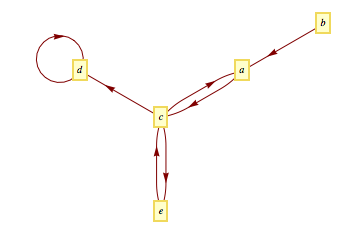
\includegraphics[width=0.5\textwidth]{2-a}
\caption{$R = \{(a,c),(b,a),(c,a),(c,d),(c,e),(d,d),(e,c)\}$}
\end{figure}

\begin{figure}[hp]
\centering
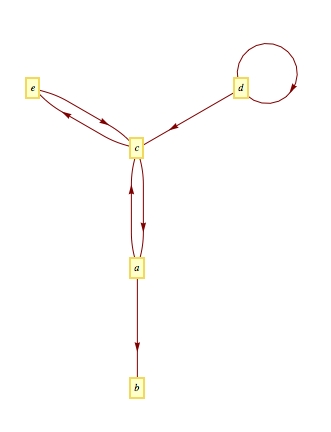
\includegraphics[width=0.5\textwidth]{2-b}
\caption{$R^{-1} = \{(c,a),(a,b),(a,c),(d,c),(e,c),(d,d),(c,e)\}$}
\end{figure}

\begin{figure}[hp]
\centering
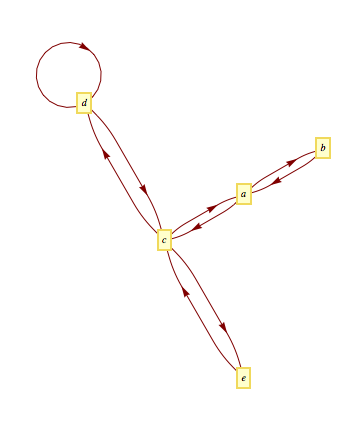
\includegraphics[width=0.5\textwidth]{2-c}
\caption{$R\cup R^{-1} = \{(c,a),(a,b),(b,a),(a,c),(c,d),(d,c),(e,c),(d,d),(c,e)\}$}
\end{figure}

\begin{figure}[hp]
\centering
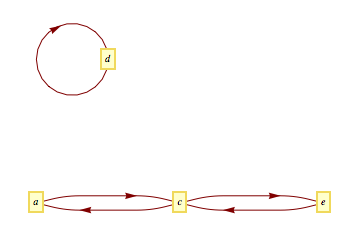
\includegraphics[width=0.5\textwidth]{2-d}
\caption{$R\cap R^{-1} = \{(a,c),(c,a),(d,d),(e,c),(c,e)\}$}
\end{figure}


%-----------------------------------------------------------------------------
% PROBLEM 3
%-----------------------------------------------------------------------------
\section{}

\begin{fancyquotes}
Fun with sets of functions:
\end{fancyquotes}

\subsection{} % (fold)
\begin{fancyquotes}
(1 point) How many different functions are there from set $\{a\}$ to the set $\{0,1\}$?
\end{fancyquotes}

It is two functions $\{a\rightarrow 0, a\rightarrow 1\}$.
% subsection  (end)

\subsection{} % (fold)
\begin{fancyquotes}
(1 point) How many different functions are there from set $\{a,b\}$ to the set $\{0,1\}$?
\end{fancyquotes}

There is four functions $\{(a\rightarrow 0, b\rightarrow 0),(a\rightarrow 0, b\rightarrow 1),(a\rightarrow 1, b\rightarrow 0),(a\rightarrow 1, b\rightarrow 1)\}$.
% subsection  (end)

\subsection{} % (fold)
\begin{fancyquotes}
(1 point) How many different functions are there from the set $A$ (where $|A| = n$) to the set $\{0,1\}$?
\end{fancyquotes}

There is $2^n$ functions.
% subsection  (end)

\subsection{} % (fold)
\begin{fancyquotes}
(1 point) How many different functions are there from the set $A$ (where $|A| = n$) to the set $B$ (where $|B| = n$)?
\end{fancyquotes}

There is $n^n$ functions.
% subsection  (end)

\subsection{} % (fold)
\begin{fancyquotes}
(3 points) Let $\{0,1\}^A$ be the set of all functions from the set $A$ to the set $\{0,1\}$
(So, $\{0,1\}^{\{a,b\}}$ would be: $\{\{(a,0),(b,0)\},\{(a,0),(b,1)\},\{(a,1),(b,0)\}...\}$.
Give a bijection between the elements of $\{0,1\}^A$ and $2^A$.
\end{fancyquotes}

Take $\{(a_1,b_1), (a_2,b_2), (a_3,b_3),...,(a_n,b_n)\}$ as a element in $\{0,1\}^A$, which $b_n \in \{0,1\}$.
Serialize/map this as $(b_1,b_2,b_3,...,b_n)$. We will get $2^n$ different serials.
Since $\{0,1\}^A$ is the set contains all possible function between $A$ and $\{0,1\}$, it is a bijection between the serials and the elements.

Also, take $\{a_2,a_3,a_7,a_{20}...,a_n\}$ is a element in $2^A$.
Then, map it to $(b_1,b_2,b_3,...,b_n)$, in which $b_i=1$ if $a_i$ in the set, otherwise $b_i=0$. This is also a bijection map.

Composite these two bijections we will get a bijection between $\{0,1\}^A$ and $2^A$.
% subsection  (end)


%-----------------------------------------------------------------------------
% PROBLEM 4
%-----------------------------------------------------------------------------
\section{}

\begin{fancyquotes}
(4 points) Draw graphical represetations of the following types of relations:
\end{fancyquotes}

\begin{figure}[hp]
\centering
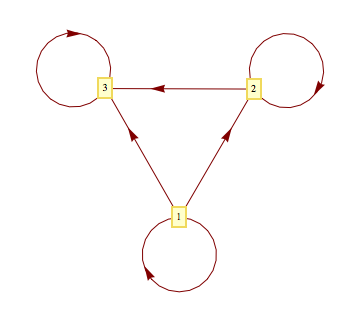
\includegraphics[width=0.5\textwidth]{4-a}
\caption{Reflexive, Transitive, Antisymmetric}
\end{figure}

\begin{figure}[hp]
\centering
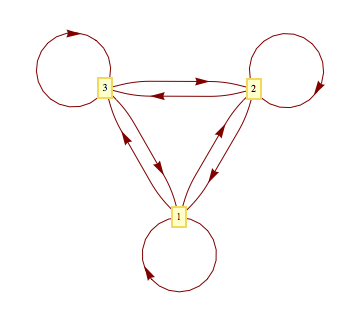
\includegraphics[width=0.5\textwidth]{4-b}
\caption{Reflexive, Transitive, Symmetric}
\end{figure}

\begin{figure}[hp]
\centering
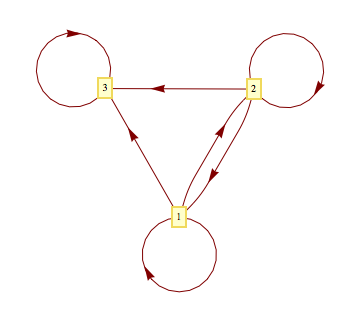
\includegraphics[width=0.5\textwidth]{4-c}
\caption{Reflexive, Transitive, neither Symmetric not Antisymmetric}
\end{figure}

\begin{figure}[hp]
\centering
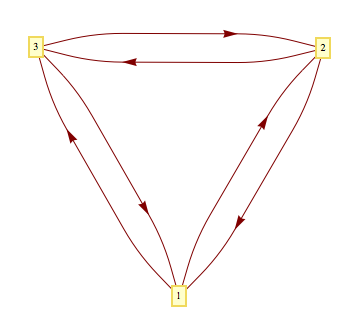
\includegraphics[width=0.5\textwidth]{4-d}
\caption{Transitive, Symmetric, and not Reflexive}
\end{figure}


%-----------------------------------------------------------------------------
% PROBLEM 5
%-----------------------------------------------------------------------------
\section{}

\begin{fancyquotes}
Let $S$ be any set, and let $P$ be the set of all partitions of $S$.
Let $R$ be the binary relation on $P$ such that $(\Pi_1, \Pi_2) \in R$ if and only if, for every $S_1 \in \Pi_1$, there is an $S_2 \in \Pi_2$ such that $S_1 \subseteq S_2$.
\end{fancyquotes}

\subsection{} % (fold)
\begin{fancyquotes}
(2 points) Give a directed graph representation of $R$ for the set $S=\{a,b,c\}$.
\end{fancyquotes}

\begin{figure}[hp]
\centering
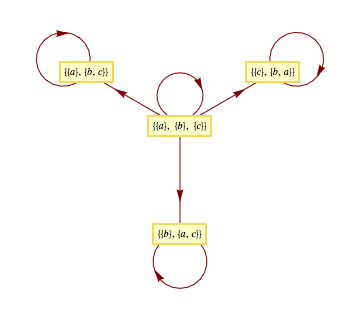
\includegraphics[width=0.5\textwidth]{5-1}
\caption{$R$ for the set $S=\{a,b,c\}$}
\end{figure}
% subsection  (end)

\subsection{} % (fold)
\begin{fancyquotes}
(2 points) Show that $R$ is a partial order on $P$ (for the general case, not just example (a) above)
\end{fancyquotes}

\subsubsection{Reflexive}
For $\forall \Pi_0 \in P$, obvioursly for $\forall S_0 \in \Pi_0$, we have $S_0 \subseteq S_0$.
So $(\Pi_0,\Pi_0)\in R$, which means $R$ is reflexive.

\subsubsection{Transitive}
For $\forall \Pi_1,\Pi_2,\Pi_3 \in P$, which $(\Pi_1,\Pi_2)\in R, (\Pi_2,\Pi_3)\in R$, we have $\forall S_1\in\Pi_1, \exists S_2, S_1\in S_2$ and $\forall S_2\in\Pi_2, \exists S_3, S_2\in S_3$.
So we have $\forall S_1\in\Pi_1, \exists S_3, S_1\in S_3$, which means $(\Pi_1,\Pi_3)\in R$.
So $R$ is transitive.

\subsubsection{Antisymmetric}
Considering any $(\Pi_1,\Pi_2)\in R$
Assume that $(\Pi_2,\Pi_1)\in R$ also.

Then $\forall s_1\in\Pi_1, \exists s_2\in\Pi_2, \exists s_3\in\Pi_1, s_1 \subseteq s_2 \subseteq s_3$.
Since $s_1 \subseteq s_3$, then we have $s_1 \cap s_3=s_1\neq \emptyset$ which means $\Pi_1$ is not a partition of $S$.

So the assumption of $(\Pi_2,\Pi_1)\in R$ is wrong.

So, for $\forall (\Pi_1,\Pi_2)\in R, (\Pi_2,\Pi_1)\notin R$, which means $R$ is antisymmetric.

So, $R$ is a partial order on $P$.
% subsection  (end)

\subsection{} % (fold)
\begin{fancyquotes}
(2 points) What elements of $P$ are maximal and minimal (for the general case, not just example (a) above)
\end{fancyquotes}

$\{\{a\}:a\in P\}$ is the minimal.

$\{S\}$ is the maximal.
% subsection  (end)

\subsection{} % (fold)
\begin{fancyquotes}
(2 points) Suppose that $P$ was an arbitrary collection of subsets of $2^S$, instead of partitions of $S$. Would $R$ still necessarily be a partial order?
\end{fancyquotes}

Considering two elements of $P$, $\Pi_1,\Pi_2\in P \subseteq 2^A$, which $S\in \Pi_1,\Pi_2$.

So, for $\forall s_1\in\Pi_1,\exists S\in\Pi_2, s_1\subset S$, which means $(\Pi_1,\Pi_2)\in R$.
Similarly, $\forall s_2\in\Pi_2,\exists S\in\Pi_1, s_2\subset S$, which means $(\Pi_2,\Pi_1)\in R$. In such a situation, $R$ is not antisymmetric.

So $R$ does not necessarily be a partial order
% subsection  (end)

\end{document}
